%%%%%%%%%%%%%%%%%%%%%%%%%%%%%%%%%%%%%%%%%%%%%%%
%%% Template for ICSI-499 Capstone Project Report
%%%%%%%%%%%%%%%%%%%%%%%%%%%%%%%%%%%%%%%%%%%%%%%

% \documentclass[12pt,english, openany]{book}
\documentclass[12pt]{article}


\usepackage[]{graphicx}
\usepackage[]{color}
\usepackage{alltt}
\usepackage[T1]{fontenc}
\usepackage[utf8]{inputenc}
\setcounter{secnumdepth}{3}
\setcounter{tocdepth}{3}
\setlength{\parskip}{\smallskipamount}
\setlength{\parindent}{0pt}

% Set page margins
\usepackage[top=100pt,bottom=100pt,left=68pt,right=66pt]{geometry}

% Package used for placeholder text
\usepackage{lipsum}

% Prevents LaTeX from filling out a page to the bottom
\raggedbottom

% Adding both languages
\usepackage[english, italian]{babel}

% All page numbers positioned at the bottom of the page
\usepackage{fancyhdr}
\fancyhf{} % clear all header and footers
\fancyfoot[C]{\thepage}
\renewcommand{\headrulewidth}{0pt} % remove the header rule
\pagestyle{fancy}

% Changes the style of chapter headings
\usepackage{titlesec}
\titleformat{\chapter}
   {\normalfont\LARGE\bfseries}{\thechapter.}{1em}{}
% Change distance between chapter header and text
\titlespacing{\chapter}{0pt}{50pt}{2\baselineskip}

% Adds table captions above the table per default
\usepackage{float}
\floatstyle{plaintop}
\restylefloat{table}

% Adds space between caption and table
\usepackage[tableposition=top]{caption}

% Adds hyperlinks to references and ToC
\usepackage{hyperref}
\hypersetup{hidelinks,linkcolor = black} % Changes the link color to black and hides the hideous red border that usually is created

% If multiple images are to be added, a folder (path) with all the images can be added here 
\graphicspath{ {Figures/} }

% Separates the first part of the report/thesis in Roman numerals
%\frontmatter


%%%%%%%%%%%%%%%%%%%%%%%%%%%%%% Starts the document
\begin{document}

%%% Selects the language to be used for the first couple of pages
\selectlanguage{english}

%%%%% Adds the title page
\begin{titlepage}
	\clearpage\thispagestyle{empty}
	\centering
	\vspace{1.5cm}
   {\normalsize
    \textbf{ICSI499 Capstone Project Report} \par
}
  	\vspace{1.5cm}
	% Titles
	{\Huge \textbf{Meal Planner App}} \\
	\vspace{3cm}
	{\normalsize \textit{Project Team}\\
		\vspace{0.25cm}
	Bhanu Kakulla   \\ % \\ specifies a new line
    Joseph Lohman	 \\
    Enoch Oluwasogo Awofeso	 \\
    Sandeep Vepuri	 \\
	............................. \\
	College of Engineering and Applied Sciences\\
	University at Albany, SUNY \par}
	\vspace{4cm}
 
    {\normalsize
    \textit{Project Sponsor}\\
    		\vspace{0.25cm}
    Dr.Pradeep Atrey  \\
    University at Albany \\
    University at Albany - State University of New York \par
}

 
    \vspace{3cm}
		
	% Set the date
	{\normalsize May 5, 2024 \par}
	
	\pagebreak


\end{titlepage}
	
\clearpage\thispagestyle{empty}

	\vspace{1cm}
		\begin{center}
\textbf{Acknowledgements}\\
		\end{center}
	\vspace{1cm}
{\normalsize As a team, we express our deepest gratitude to Professor Pradeep Atrey for his invaluable support and guidance throughout the development of our Meal Planner App. Professor Atrey's mentorship, regular meetings, and structured checkpoints played a pivotal role in shaping our project's direction and ensuring its success. We as a team were able to coordinate and have a projection of our goals and milestones to be completed. We are truly honored to have had the opportunity to collaborate with him on this endeavor. It was a honor to create the Meal Planner App!
\par}

\clearpage\thispagestyle{empty}

	\vspace{1cm}
		\begin{center}
\textbf{Abstract}\\
		\end{center}
	\vspace{1cm}
{\normalsize The Meal Planner App is a Android-based application aimed at simplifying meal planning and enhancing user experience. Leveraging data from the Spoonacular API, the app offers personalized meal suggestions based on user preferences and dietary requirements. Users can register and manage their profiles seamlessly, allowing for customization of meal plans and preferences. The app's intuitive user interface guides users through the process of selecting, saving, and exploring meal options with ease. Backed by robust algorithms and tools, the Meal Planner App aims to revolutionize the way users approach meal planning, creating culinary creativity in how the user prepares for cooking.\par}
\clearpage\thispagestyle{empty}
% Adds a table of contents
\tableofcontents{}
\clearpage\thispagestyle{empty}
%%%%%%%%%%%%%%%%%%%%%%%%%%%%%%%%%%%%%%%%%%%%%%%%%%%%%%%%%%%%%%%%%%%%%%%%%%%%%%%%%%%%%%%%%%%%
%%%%%%%%%%%%%%%%%%%%%%%%%%%%%%%%%%%%%%%%%%%%%%%%%%%%%%%%%%%%%%%%%%%%%%%%%%%%%%%%%%%%%%%%%%%%
%%%%% Text body starts here!
%\mainmatter

\section{Problem Analysis}\label{chap:introduction}
    \item Meal planning can be a time-consuming and daunting task for many individuals, especially those with dietary restrictions or specific health goals. The problem we aim to address with the Meal Planner App is the lack of efficient and personalized tools to streamline the meal planning process and provide users with tailored meal suggestions. This problem is significant as it directly impacts users' daily routines, health outcomes, and overall well-being. Moreover, with the growing emphasis on healthy eating and the increasing prevalence of dietary restrictions, there is a growing need for accessible and user-friendly solutions in the realm of meal planning.
\subsection{Existing solutions}
Existing solutions for meal planning often lack personalization, relying on generic meal suggestions that may not align with individual preferences or dietary requirements. Furthermore, these solutions may not offer seamless integration with user profiles, making it challenging for users to manage their meal preferences and track their progress effectively. Key weaknesses of existing solutions include limited customization options, lack of real-time updates, and insufficient support for dietary restrictions.

\subsection{Core Idea and Solution}
The core idea of our solution is to provide users with a user-friendly, customizable meal planning app that integrates seamlessly with their dietary preferences and cooking expertise. Key characteristics of our proposed solution include personalized meal recommendations, real-time updates, and comprehensive support for various dietary restrictions.

Our solution stands out from existing ones by offering a higher level of personalization, integration with user profiles, and the ability to tailor meal suggestions based on individual preferences and cooking expertise. Furthermore, our app provides a wide range of meal options, addressing the limitations of current solutions.
\subsection{Key Contributions}
- Streamlining the meal planning process for users with diverse dietary preferences and restrictions.
\\- Enhancing user satisfaction and adherence to dietary goals through personalized meal suggestions.
\\- Providing a user-friendly interface and seamless integration with user profiles for efficient meal management.
\subsection{Organization of this Report}
This report is structured to provide a comprehensive overview of the problem domain, existing solutions, our proposed solution, its novelty and distinctiveness, key contributions, and the organization of the project. Each section builds upon the previous one to present a cohesive understanding of the project's scope and objectives.




\section{Proposed System/Application/Study}\label{chap:proposed}

\textbf{Length of this section should be 1000-1500 words.}

\subsection{Overview} 
($\approx$100 words)\\
Provide an overview of the proposed system/application/study. Also, state how this whole section is organized, and what the readers should expect next.

\subsection{Project Requirements}\label{sec:requirements}
($\approx$500 words)\\
In this section, you will provide descriptions of all requirements of the proposed system/application, mostly what did in Milestone 2, part 2, but possibly more detailed, as needed. Specifically, it should include the following: User Class and Functional Requirements, Non- Functional Requirements, Operating Requirements, and Design and Implementation Constraints.

\subsection{Technical Design}\label{sec:design}
($\approx$500 words)\\
Describe your technical solution. Include high-level drawings and illustrations that can help
the reader under the system. Provide use-case diagrams, system architecture and data flow diagrams (Figure \ref{fig:simulationfigure} and appropriately discuss them in the text. This is mostly what you did in Milestone 4, but possibly more detailed, as needed.

\begin{figure}[h]
    \centering
    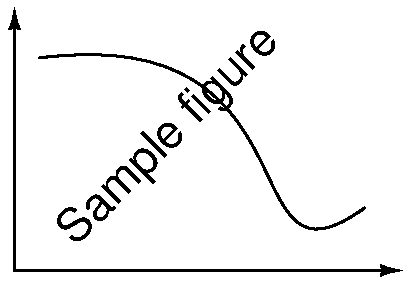
\includegraphics[height = 2.0in, width=3.0in]{myfigure}
    \caption{Simulation Results}
    \label{fig:simulationfigure}
\end{figure}

\subsection{System Implementation}\label{chap:implementation}
($\approx$150 words)\\
In this section, you will provide the details of system implementation, such as programming tools and development environment, libraries. Provide some snapshots of the system/application/GUI.

\subsection{Use of Computer Science Theory and Software Development Fundamentals}\label{chap:theory_sw} 
($\approx$250 words)\\

In this section, you will discuss the use of computer science theories and software development fundamentals in your project.
You are required to explicitly state three instances of application of computer science theories and software development fundamentals each and explain where and how exactly you have used it. Examples of computer science theories may include specific data structures or known algorithms that you may have used, computational complexity analysis of any subproblem that you may have solved, during the course of the project, and database design and normalization. Software development fundamentals may include efficient use of design patterns, modular and reusable coding practices, code documentation, unit testing, and integration tools. Please use the following template:

\subsubsection{Use of Computer Science Theories}
Some text...
\begin{description}
    \item [Name of CS theory 1] Describe a specific instance of CS theory 1 here.
    \item [Name of CS theory 2] Describe a specific instance of CS theory 2 here.
    \item [Name of CS theory 3] Describe a specific instance of CS theory 3 here.
\end{description}

\subsubsection{Use of Software Development Fundamentals}
Some text.
\begin{description}
    \item [Name of software development fundamental 1] Describe a specific instance of software development fundamental 1 here.
    \item [Name of software development fundamental 2] Describe a specific instance of software development fundamental 2 here.
    \item [Name of software development fundamental 3] Describe a specific instance of software development fundamental 3 here.
\end{description}

\section{Experimental Design and Testing}\label{chap:results}

\textbf{Length of this section should be 1000-1500 words.}\\

Design meaningful tests that ensure that your system is solving the stakeholder’s problem (validation) and being built correctly (Verification). 

In this section, you must provide the following section in sufficient detail.
\subsection{Experimental Setup}\label{sec:exp_setup}
    \begin{itemize}
        \item State the objectives of experiments – what and why do we want to perform experiments?
        \item Layout the number of experiments (Experiment \#1, \#2, etc.).
        \item Describe the experimental setup (machine/system and devices used, lab or real-world environment, etc.) for each experiment.
    \end{itemize}
\subsection{Dataset}\label{sec:dataset}
        Describe the dataset (size of data, how collected: is it publicly available, obtained from an organization, or collected via users (if users, how many users, who were the users - no identity disclosure without written consent)) for each experiment. 

\subsection{Results and Analysis}\label{sec:results}
    \begin{itemize}
        \item Present the results and analysis using figures, graphs, and tables (like Table \ref{tab:relatedwork} below), as appropriate for your work, and adequately discuss them in the text.

\begin{table}[h]
\begin{center}
\caption{Existing work}\label{tab:relatedwork}
\begin{tabular}{|l|c|l|l|l|}
\hline
Name & Age & Qualification & City & Phone\\
\hline
Pradeep & 25 & PhD & Albany & 91023910\\
XXX  & 25 & PhD & Albany & 91023910\\
\hline
\end{tabular}
\end{center}
\end{table}
        \item Justify/argue how your results are better than the existing systems/applications/ studies at least in some aspect(s).
 \item	Identify the expected, and most importantly “unexpected”, findings from the experiments.
 \item	Identify the `wow' factor from the experiments (if possible).
 \item	Failure cases
    \begin{itemize}
        \item Describe the anticipated limitations of your system/application.
        \item Your system/application may not work in all conditions and for all inputs – identify and discuss the conditions or situations when it may fail, and how you plan to validate it.
    \end{itemize}
\end{itemize}



\section{Legal and Ethical Practices}\label{chap:ethics}
($\approx$300 words)\\
Discuss the most important ethical and legal considerations that arose, and more importantly, how these were addressed in your project. These can vary dramatically from project to project. This section must include two subsections, as given below.
\subsection{Legal Considerations}\label{sec:legal}
\begin{itemize}
\item Intellectual property concerns regarding the ownership of the underlying technology, as well as potential copyright or trademark concerns.
\end{itemize}

\subsection{Ethical Considerations}\label{sec:ethical}
\begin{itemize}
\item Informed consent regarding data leverage users or testers.
\item Privacy concerns with your proposed system, including the use of personally identifiable
data.
\item Consideration and mitigation of any risks that might arise in the use of your proposed
system.
\item Intellectual property concerns regarding the ownership of the underlying technology,
as well as potential copyright or trademark concerns.
\end{itemize}


\section{Effort Sharing}\label{chap:conclusion}
($\approx$200 words)\\
Since it is a team-based project, team members must explicitly state their separate efforts/ contributions in addition to the joint efforts. This section must clearly state how different tasks of the project were divided into  team members, and who did what (as shown in Table \ref{tab:effortsharing}). 
\begin{table}[h]
\begin{center}
\caption{Effort sharing}\label{tab:effortsharing}
\begin{tabular}{|c|c|c|c|c|c|c|}
\hline
Team size & Joint efforts & Member 1 & Member 2 & Member 3 & Member 4 & Member 5\\
\hline
5 & J ($\approx$25\%) & I ($\approx$15\%) & I ($\approx$15\%) & I ($\approx$15\%) & I ($\approx$15\%) & I ($\approx$15\%)\\
4 & J ($\approx$30\%) & I ($\approx$17.5\%) & I ($\approx$17.5\%) & I ($\approx$17.5\%) & I ($\approx$17.5\%) & -\\
3 & J ($\approx$31\%) & I ($\approx$23\%) & I ($\approx$23\%) & I ($\approx$23\%) & - & -\\
2 & J ($\approx$40\%) & I ($\approx$30\%) & I ($\approx$30\%) & - & - & -\\
\hline
\end{tabular}\\
J = description of tasks jointly performed\\
I = description of tasks individually performed
\end{center}
\end{table}


\section{Conclusion and Future Work}\label{chap:conclusion}
($\approx$150 words)\\
State what you conclude from this work and what are the future work possibilities.


\textbf{Provide below at least 10-15 references for your work.}
% Adding a bibliography if citations are used in the report
\bibliographystyle{plain}
\bibliography{bibliography.bib}
% Adds reference to the Bibliography in the ToC
\addcontentsline{toc}{chapter}{\bibname}

\pagebreak




\end{document}
